\section{Pattern}

\subsection{Equipment-Erzeugung mittels Fabrik}
Da die Equipments der Spieler unterschiedlich sein k�nnen und auch in der Zukunft erweiterbar sein sollen, werden sie
von einer Fabrik-Klasse erzeugt. Die Equipments m�ssen in Client und Server jedoch unterschiedliche Implementierungen
haben. Im Client soll das Equipment grafisch dargestellt und Sounds abgespielt werden. Im Server dagegen soll
stattdessen die Auswirkungen der Benutzung berechnet werden. Daher kommt hier das Abstrakte-Fabrik-Muster zum Einsatz.
Das Abstrakte-Fabrik-Muster setzt Spezifikationsvererbung ein, um die Schnittstelle eines Produkts von seiner
Implementierung zu entkoppeln. Um sicherzustellen, dass auf jeder Plattform stets nur die richtigen Objekte erzeugt
werden, also eine konsistente Menge von Objekten vorhanden ist, d�rfen Objekte nur �ber eine Fabrik erzeugt
werden\cite{Bruegge_2004}. Im Fall der Equipments existiert eine ClientEquipmentFactory und eine ServerEquipmentFactory
die jeweils die von AbstractEquipmentFactory geerbten Methoden zur Erzeugung von Pick'n'Place- und Swapper-Equipments
implementieren. Abbildung \ref{equipment_factory} zeigt die Struktur als UML-Klassendiagramm.

\begin{figure}[htbp]
\centering
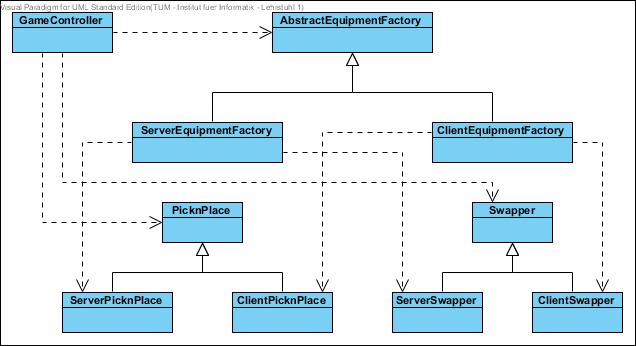
\includegraphics[width=1.0\textwidth]{images/equipment_factory}
\caption[UML-Klassendiagramm: Equipment-Factory]{UML-Klassendiagramm: Equipment-Factory}
\label{equipment_factory}
\end{figure}

\subsection{Szenen-Graph-Erstellung mithilfe des Kompositionsmusters}
Wie bereits erw�hnt, besteht die Spielwelt aus vielen einzelnen Objekten. Die jMonkeyEngine3 organisiert die Objekte f�r
das Rendering in einer hierarchischen Baumstruktur, dem "`scene graph"'. Dieser ist ein gerichteter azyklischer Graph,
wie ihn die meisten Graphik-Engines nutzen\cite{???}. Das Kompositionsmuster ist eine L�sung, um eine Hierarchie
beliebiger Breite und Tiefe zu repr�sentieren, sodass sowohl einzelne Objekte als auch Kompositionen von Objekten durch
eine gemeinsame Schnittstelle einheitlich behandelt werden k�nnen. Abbildung \ref{composition_spatial} zeigt die
Umsetzung des Kompositionsmusters in der jMonkeyEngine3. Die Komponente-Klasse ist hier Spatial und Geometry ist die
Blatt-Klasse. Sie stellt ein tats�chliches Objekt in der virtuellen Welt dar, definiert durch Formen und Materialien.
Die Kompositum-Klasse ist Node, welche wiederum andere Spatials als Kindelemente enthalten kann.\\

\begin{figure}[htbp]
\centering
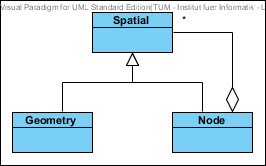
\includegraphics[width=0.6\textwidth]{images/composition_spatial}
\caption[UML-Klassendiagramm: Implementierung des Kompositionsmuster im Szenen-Graph der jME3]{UML-Klassendiagramm: Implementierung des Kompositionsmuster im Szenen-Graph der jME3}
\label{composition_spatial}
\end{figure}

Ein Beispiel f�r die Zusammensetzung der virtuellen Welt aus Spatials, kann anhand des Avatars eines Spieler gegeben
werden. Abblidung \ref{composition_avatar} veranschaulicht die Struktur der Spielfigur. Der Wurzelknoten hat drei
Kindelemente: Kopf, Oberk�rper, Unterk�rper. Der Kopf ist vom Typ Geometry, w�hrend Ober- und Unterk�rper Nodes sind,
die wiederum Kindelemente besitzen, n�mlich Arme, Beine und Torso. Die Unterteilung k�nnte nat�rlich auch noch weiter
gehen: ein Arm k�nnte zum Beispiel wiederum ein Knoten sein, der aus Oberarm, Unterarm und Hand, besitzt, wobei die Hand
ebenfalls aus einzelnen Fingern bestehen k�nnte, usw. Beliebig feingliedrige Strukturen sind m�glich, je nach
gew�nschtem Detailgrad der Modelle.

\begin{figure}[htbp]
\centering
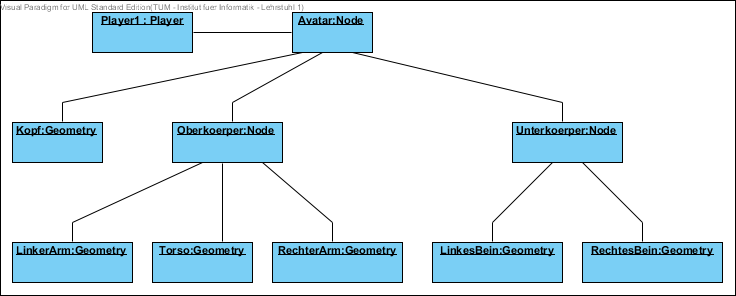
\includegraphics[width=1.0\textwidth]{images/composition_avatar}
\caption[UML-Objektdiagramm: Aufbau des Spieler-Modells]{UML-Objektdiagramm: Aufbau des Spieler-Modells}
\label{composition_avatar}
\end{figure}
